%----------------------------------------------------------------------------------------
%	Metropolia Thesis LaTeX Template
%----------------------------------------------------------------------------------------
% License:
% This work is licensed under the Creative Commons Attribution 4.0 International License. 
% To view a copy of this license, visit http://creativecommons.org/licenses/by/4.0/.
%
% However, this license apply to this template. As a template, it is supposed to be 
% modified for your own needs (with your thesis content). For this reason, if you use 
% this project as a template and not specifically distribute it as part of a another 
% package/program, we grant the extra permission to freely copy and modify these files as 
% you see fit and even to delete this copyright notice. 
% In short, you are free to publish your thesis under whatever license you wish, even 
% keep the all rights reserved to you.
%
% Authors:
% Panu Leppäniemi, Patrik Luoto and Patrick Ausderau
%
% Credits:
% Panu Leppäniemi: abstract, def, cleaning,...
% Patrik Luoto: title page, abstract in Finnish, abbreviation, math,...
% Patrick Ausderau: initial version, style, table of content, bibliography, figure, 
%                   appendix, table, source code listing...
%
% Please:
% If you find mistakes, improve this template and alike, please contribute by sharing 
% your improvements and/or send us your feedback there: 
% https://github.com/panunu/metropolia-thesis-latex
% And of course, if you improve it, add yourself as an author.
%
% Compiler:
% Use XeLaTeX as a compiler.
 
%----------------------------------------------------------------------------------------
%	THESIS INFO
%----------------------------------------------------------------------------------------

% All general information (main language, title, author (you), degree programme, major 
% option, etc.)
% Edit the file chapters/0info.tex to change these information
% Global information (title of your thesis, your name, degree programme, major, etc.) 

% Yifan: keep it as finnish, otherwise there'll be compilation error
\def\thesislang{finnish} %change this depending on the main language of the thesis.
% "english" is the only other supported language currently. If someone has the swedish, please contribute!

\def\secondlang{english} %if the main language is Finnish (or Swedish), you must have 2 abstracts (one in Finnish (or Swedish) and one in English)
%If the main language is English and that you are native Finnish (or Swedish) speaker, you must have also abstract in your native language on top of the English one.

\author{Yifan Yu} %your first name and last name
\def\thesis{Thesis}%keep the half based on the main thesis language
%was Opinnäytetyö

\def\alaotsikko{} %if you don't have subtitle, empty {} it (but don't delete that line)

%Finnish section, for title/abstract
\def\otsikko{Implementing the Generator of DCGAN on FPGA (Draft)}
\def\tutkinto{Bachelor of Engineering} % change to your needs, e.g. "YAMK", etc.
\def\kohjelma{Electronics}
\def\suuntautumis{}
\def\ohjaajat{
Janne Mäntykoski, Senior Lecturer
}
\def\avainsanat{FPGA, Generative Adversarial Networks, Deep Learning}
\def\pvm{\specialdate\today}

%English section, for title/abstract
\title{Implementing the Generator of DCGAN on FPGA}
\def\metropoliadegree {Bachelor of Engineering} % change to your needs, e.g. "master", etc.
\def\metropoliadegreeprogramme {Electronics}
\def\metropoliaspecialisation {}
\def\metropoliainstructors {
Janne Mäntykoski, Senior Lecturer
}
\def\metropoliakeywords {FPGA, Generative Adversarial Networks, Deep Learning}
\date{\longmonth\today}




%----------------------------------------------------------------------------------------
%	GLOBAL STYLES
%----------------------------------------------------------------------------------------

% If you need extra package, etc. modify the style/style.tex file.
% If you are using Windows OS, you will need to change default font to Arial in that 
% style/style.tex file (or install Liberation Sans font to your system).
% If you are using MacOS or linux, make sure you have Liberation Sans font installed.
% Global style. Normally should not be edited. 
% If you use windows OS, eventually change \setmainfont to Arial
% Check around commit https://github.com/panunu/metropolia-thesis-latex/commit/a0c15ac77bab1a52c59c517a18080938e57bf5ef
% to see how the font files were manually added (after downloading them: https://pagure.io/liberation-fonts/ )

\documentclass[11pt,a4paper,oneside,article]{memoir}
\usepackage[\secondlang,\thesislang]{babel}% finnish english swedish
\usepackage{iflang}
\usepackage{amsmath}
\usepackage{amsfonts}
\usepackage{amssymb}
\usepackage{fontspec}
\usepackage{tocloft}
\usepackage{titlesec}
\usepackage[hyphens]{url}
\usepackage{mathtools}
\usepackage{wallpaper}
\usepackage{datetime}
\usepackage[bookmarksdepth=subsection,hidelinks]{hyperref} % for automagic pdf links for toc, refs, etc.
\usepackage[amssymb]{SIunits}
\usepackage[version=3]{mhchem}
\usepackage{pgfplots} %simple plots etc
\usepackage{pgfplotstable}
\usepackage{tikz} % mindmaps, flowcharts, piecharts, examples at http://www.texample.net/tikz/examples/
\usetikzlibrary{shapes.geometric, arrows}


\renewcommand{\dateseparator}{.}
%condition for adding or not space in TOC
\usepackage{etoolbox}
%for compact list
\usepackage{enumitem}
%for block comment
\usepackage{verbatim}
%for "easier" references
\usepackage{varioref}
%forcing single line spacing in bibliography
\DisemulatePackage{setspace}
\usepackage{setspace}
%including figure (image)
\usepackage{graphicx}
%change the numbering for figure
\usepackage{chngcntr}
%strike trough
\usepackage{ulem}
%euro symbol
\usepackage{eurosym}
%try to count
\usepackage{totcount}
%insert source code
%\usepackage{listings}
%require -8bit -shell-escape in the xelatex compile command
\usepackage[newfloat]{minted}
\setminted{tabsize=2,linenos,breaklines,breaksymbolleft={\quad},baselinestretch=1}
\setmintedinline{breaklines}
\usepackage[justification=justified,singlelinecheck=false]{caption}
\usepackage{color}
%force the width of a table instead of column
\usepackage{tabularx}
\usepackage{booktabs} %why not booktabs? :3
% Abbreviations, acronym and glossary
\usepackage[acronym,nonumberlist,section]{glossaries}%xindy,%toc, ,nomain

\usepackage{float} % For forced figure location with modifier H (\begin{figure}[H])
\usepackage{cite} % Make citations to match Metropolia thesis guide

% change font of links in bibliography to same as other text
\usepackage{url}
\urlstyle{same}

% change punctuation of multiple cites to semicolon instead of comma: [1; 2; 3]
\renewcommand\citepunct{; }

% citep-macro for reference with period inside square brackets [1.]
\newcommand{\citep}[1]{
 \renewcommand\citeright{.]}
 \cite{#1}
 \renewcommand\citeright{]}
}

%set date format to D.M.YYYY
\newdateformat{specialdate}{\THEDAY.\THEMONTH.\THEYEAR}
%set date format to D Month YYYY
\newdateformat{longmonth}{\THEDAY~\monthname[\THEMONTH] \THEYEAR}

\newcommand\tn[1]{\textnormal{#1}} %use \tn instead of \textnormal
\newcommand\reaction[1]{\begin{equation}\ce{#1}\end{equation}} %\reaction{} for chemical reactions

%NORMAL TEXT
%all text, title, etc. in the same font: Arial
%NOTE: fontname is case-sensitive
\setmainfont{Liberation Sans}
%line space
\linespread{1.5}
\AtBeginEnvironment{tabular}{\singlespacing}
%\doublespacing
%margin
\usepackage[top=2.5cm, bottom=3cm, left=4cm, right=2cm, nofoot]{geometry}
\setlength{\parindent}{0pt} %first line of paragraph not indented
\setlength{\parskip}{16.5pt} %one empty line to separate paragraph
%list with small line space separation
\tightlists

%IMAGE - FIGURE
%the figures should be placed in the "illustration" folder
\graphicspath{{illustration/}}
%figure number without chapter (1.1, 1.2, 2.1) to (1, 2, 3)
\counterwithout{figure}{chapter}
%border around images
\setlength\fboxsep{0pt}
\setlength\fboxrule{0.5pt}
%caption font size
\captionnamefont{\small}
\captiontitlefont{\small}
%space after figure caption (and other float elements)
\setlength{\belowcaptionskip}{-7pt}

%TABLE
\counterwithout{table}{chapter}

%SOURCE CODE
\newenvironment{code}{\captionsetup{type=listing}}{}
\IfLanguageName {finnish} {\SetupFloatingEnvironment{listing}{name=Listing}} {}
%\counterwithout{lstlisting}{chapter}
%moved after begin document, otherwise does not compile

%% set this format as the default for lstlisting
%\DeclareCaptionFormat{empty}{}
%\captionsetup[lstlisting]{format=empty}

%TOC
%change toc title
\IfLanguageName {finnish} {\addto{\captionsfinnish}{\renewcommand*{\contentsname}{Contents}}} {}
%remove dots
\renewcommand*{\cftdotsep}{\cftnodots}
%chapter title and page number not in bold
\renewcommand{\cftchapterfont}{}
\renewcommand{\cftchapterpagefont}{}
%sub section in toc
\setcounter{tocdepth}{2}
%subsection numbered
\setcounter{secnumdepth}{2}
\renewcommand{\tocheadstart}{\vspace*{-15pt}}
\renewcommand{\printtoctitle}[1]{\fontsize{13pt}{13pt}\bfseries #1}
\renewcommand{\aftertoctitle}{\vspace*{-22pt}\afterchaptertitle}
%spacing afer a chapter in toc
\preto\section{%
  \ifnum\value{section}=0\addtocontents{toc}{\vskip11pt}\fi
}
%spacing afer a section in toc
\renewcommand{\cftsectionaftersnumb}{\vspace*{-3pt}}
%spacing afer a subsection in toc
\renewcommand{\cftsubsectionaftersnumb}{\vspace*{-1pt}}
%appendix in toc with "Appendix " + num
\IfLanguageName {finnish} {
  \renewcommand*{\cftappendixname}{Appendix\space}
  \renewcommand{\appendixtocname}{Appendices}
}{\renewcommand*{\cftappendixname}{Appendix\space}}
%appendix header
\IfLanguageName {finnish} {\def\appname{Appendix\space}}{\def\appname{Appendix\space}}

%TITLES
%chapter title
%\clearforchapter{\clearpage}
\titleformat{\chapter}
{\fontsize{13pt}{13pt}\bfseries\linespread{1}}%\clearpage
{\thechapter}{.5cm}{}
\titlespacing*{\chapter}{0pt}{.32cm}{9pt}
\titleformat{\section}
{\fontsize{12pt}{12pt}\linespread{1}}
{\thesection}{.5cm}{}
\titlespacing*{\section}{0pt}{14pt}{6pt}
\titleformat{\subsection}
{\fontsize{12pt}{12pt}\linespread{1}}
{\thesubsection}{.5cm}{}
\titlespacing*{\subsection}{0pt}{14pt}{6pt}


%QUOTE
\renewenvironment{quote}
  {\list{}{\rightmargin=0pt\leftmargin=1cm\topsep=-10pt}%
  \item\relax\fontsize{10pt}{10pt}\singlespacing}
  {\endlist}

%BIBLIOGRAPHY
%bibliography title to be "references"
%IF THE TITLE DON'T GET RENAMED PROPERLY, move that line after the \begin{document}
\IfLanguageName {finnish} {\addto{\captionsfinnish}{\renewcommand*{\bibname}{References}}} {\renewcommand\bibname{References}}
\makeatletter %reference list option change
\renewcommand\@biblabel[1]{#1\hspace{1cm}} %from [1] to 1 with 1cm gap
\makeatother %
\setlength{\bibitemsep}{11pt}

%count the appendices (since the chapter counter is reset after \appendix).
%! require to complie 2 times
\regtotcounter{chapter}


\makepagestyle{tiivis}
\makeevenhead{tiivis}{}{}{Tiivistelmä}
\makeoddhead{tiivis}{}{}{Tiivistelmä}

\makepagestyle{abstract}
\makeevenhead{abstract}{}{}{Abstract}
\makeoddhead{abstract}{}{}{Abstract}

% Normally, you do not need to modify the title style. It's content comes from the 
% chapters/0info.tex file.
% TITLE PAGE
% Normally, you should not edit this file.

\makeatletter
\renewcommand{\maketitle}{
\thispagestyle{empty}
\ThisCenterWallPaper{1}{viiva}
%
\vspace*{9.5cm}
\tn{\LARGE\@author\\[22pt]\Huge\IfLanguageName {finnish}{\otsikko}{\@title}\\[22pt]\LARGE\alaotsikko\\[1.75cm]}

\parbox{.7\linewidth}{
\IfLanguageName {finnish}{
  Metropolia Metropolia University of Applied Sciences\\
  \tutkinto \\
  \kohjelma \\
  \thesis\\
  \pvm
} {
  Helsinki Metropolia University of Applied Sciences\\
  \metropoliadegree \\
  \metropoliadegreeprogramme \\
  \thesis\\
  \IfLanguageName {finnish}{\pvm}{\@date} % D.M.YYYY date format for Finnish. D Month YYYY for English
}
}
\ThisLRCornerWallPaper{1}{metropolia}
%
\clearpage
}
\makeatother



%----------------------------------------------------------------------------------------
%	ABBREVIATION AND GLOSSARY
%----------------------------------------------------------------------------------------

% Add/edit all your acronyms, abbreviations, glossary entries, etc. definitions in 
% chapters/0abbr.tex file.
% You can have as many as you wish. Only the ones you use in your text (inserted with 
% \gls{} command) will print in the Glossary/Lyhenteet.
% Generate the glossary
\makeglossaries

% Acronyms, abbreviations, etc. 

\newacronym{html}{HTML}{HyperText Markup Language}
\newacronym{ram}{RAM}{Random Access Memory}


% Glossary entries

\newglossaryentry{latex}
{
    name=\LaTeX{},
    description={Is a mark up language specially suited for scientific documents}
}

\newglossaryentry{maths}
{
    name=mathematics,
    description={Mathematics is what mathematicians do}
}



%----------------------------------------------------------------------------------------
%	DOCUMENT STARTS HERE...
%----------------------------------------------------------------------------------------

\begin{document}
\counterwithout{listing}{chapter}

%----------------------------------------------------------------------------------------
%	TITLE PAGE
%----------------------------------------------------------------------------------------

\input{style/title_headers.tex}
\maketitle
\newpage
%all abstract, table of content and glossary will get the metropolia logo at bottom
\LRCornerWallPaper{1}{footer}

%----------------------------------------------------------------------------------------
%	ABSTRACT / Tiivistelmä
%----------------------------------------------------------------------------------------

% If you are international student writing in English, remove the Finnish abstract.
% If you are Finnish citizen, you must have 2 abstracts, one in Finnish (or Swedish 
% depending on your mother tongue) and one in English regardless of the main language of 
% your thesis.
%\input{chapters/0abstract_fi.tex}
% Abstract in English
%Most probably, you only need to change the text of the abstract. Everything else comes from chapter/0info.tex
%If you do not have any appendix, you may delete \total{chapter} and replace with 0

\pagestyle{abstract}
\begin{otherlanguage}{english}
{\renewcommand{\arraystretch}{2}%
\begin{tabular}{ | p{4,7cm} | p{10,3cm} |}
  \hline
  Author(s) \newline
  Title \newline\newline 
  Number of Pages \newline
  Date
  & 
  \makeatletter
  \@author \newline
  \@title \newline\newline
  \pageref*{LastPage} pages + \total{chapter} appendices \newline %! if no appendices, risk to count total of chapter :D
  \IfLanguageName {finnish} {\foreignlanguage{english}{\longdate\@date}} {\@date}
  \makeatother
  \\ \hline
  Degree & \metropoliadegree
  \\ \hline
  Degree Programme & \metropoliadegreeprogramme
  \\ \hline
  Professional Major & \metropoliaspecialisation
  \\ \hline
  Instructor(s) & \metropoliainstructors
  \\ \hline
  \multicolumn{2}{|p{15cm}|}{\vspace{-22pt}
  The parallel nature of FPGA makes it a promising candidate to accelerate machine learning tasks. The
  purpose of this project was to study the acceleration capabilities of FPGA for deep convolutional
  neural networks.\newline
  
  The project was carried out by implementing a generative model on the Nexys 4 trainer board with an
  Artix-7 FPGA from Xilinx. The pre-trained model is part of the popular Generative Adversarial Networks
  (GANs) which can create realistic images that resemble the training data. The core was written in
  Verilog, but several Xilinx IPs were also used to facilitate the design. Xilinx Vivado 2017.4 was used as
  the development platform. Both fixed-point and floating-point arithmetics were used to achieve a balance
  between efficiency and accuracy.\newline
  
  With simplicity as the main goal of the design, some optimizations were deliberately avoided.
  This paper serves as a detailed documentation of the design and implementation process.
  The core operation of the generative model called transposed
  convolution is described. A method to map network weights and biases from high precision floating-point
  representation to low precision integral representation, known as quantization, is derived. The
  quantization scheme leads to an efficient implementation of the General Matrix Multiplication (GEMM) operation,
  which is at the heart of neural network computations. As a conclusion, possible optimization methods are
  discussed as future work.

  } \\[14cm] \hline
  Keywords & \metropoliakeywords
  \\ \hline
\end{tabular}
}
\end{otherlanguage}
\clearpage



%----------------------------------------------------------------------------------------
%	License? Acknowledgement?
%----------------------------------------------------------------------------------------

% Uncomment next line and edit chapters/0license.tex if you want license in your thesis.
%\input{chapters/0license.tex}

% Uncomment next line and edit chapters/0acknowledgement.tex if you want acknowledgements.
%\input{chapters/0acknowledgement.tex}

%----------------------------------------------------------------------------------------
%	TABLE OF CONTENTS
%----------------------------------------------------------------------------------------

\input{style/toc.tex}

%list of figure, tables would come here if relevant?

%----------------------------------------------------------------------------------------
%	Lyhenteet / Abbreviation
%----------------------------------------------------------------------------------------

% If you don't use abbreviations/glossary, remove the following line.
% Abbreviation and Glossary
% Normally, you don't have to modify this file. Your abbreviations, etc. goes in 
% ../chapters/0abbr.tex file.

\begin{singlespacing}

% \gsladdall would add all terms even if not used in your text.
%\glsaddall

{
	\titleformat{\section}
	{\fontsize{13pt}{13pt}\bfseries\linespread{1}}
	{\thesection}{.5cm}{}
	%Adapt labelwidth (sorry for the ugly hack)
	\setlist[description]{leftmargin=!, labelwidth=4em}
	\IfLanguageName {finnish} {
		\printacronyms[title=List of Abbreviations]
	}{
		\printacronyms[title=Abbreviations]
	}
	\setlist[description]{leftmargin=!, labelwidth=7em}
	\printglossary 
	\setlist[description]{style=standard} % reset settings back to default
}
\end{singlespacing}

\clearpage


%----------------------------------------------------------------------------------------
%	CONTENT
%----------------------------------------------------------------------------------------

\input{style/content.tex}%reset page number to 1, no more logo footer, etc.

% Thesis content if you strictly follow the "Final Year Project guide". Of course, you 
% can adapt to your specific needs (add more chapter, rename them, etc.).
% Introduction

\chapter{Introduction}

Specialized hardware for running deep learning algorithms seems to be a natural step in the evolution of
Artificial Intelligence.  Google, for exmaple, developed its own ASIC named Tensor Processing Unit (TPU)
to accelerate tensor computations. The formidable cost of such endeavors limits ASIC development to the big
players in the industry. For tech startups and hobbists, the Field Programmable Gate Array (FPGA) comes to
rescue by filling the gap between high-cost custimzed ICs and the need to make specialized hardware for certain
applications.

Generative models are a class of machine learning algorithms which, instead of processing real world data,
creates fresh and new data the world has never seen before. In other words, such algorithms enables
the machine to paint new paintings, compose new music, and write new poetries.

Generative Adversarial Networks (GANs) are a class of neural networks in which two different networks are
trained to complete against each other to learn about the probability distribution of a particular dataset.
Introduced in 2014 by Ian Goodfellow \textit{et al}., it soon gained polularity in the machine learning
community, kindled a wave of research on improving the training property and quality of generation of GANs.

The marriage of FPGA and GANs seems to be an interesting topic in its own right. The project explores such
possiblities by implementing a pre-trained generator model of GANs on the FPGA board to generate realistic
pictures. A näive version is presented first, then several optimization possibilities are explored. This
paper serves as a rather detailed documentation of the design and implementation process.

The generator is a deep Convolutional Neural Network (CNN). In such networks a large part of the computation is
done with an operation called the General Matrix Multiplication (GEMM). Therefore, an efficient implementation
of GEMM is crutial to the acceleration. However, CNNs are normally implemented with floating-point numbers,
which are much less efficient to handle in hardware than fixed-point numbers. If only we could carry out
the computation in fixed-point numbers and then convert the result back to floating-point numbers! Such
techniques do exist and they are referred to as quantization, which is the key to realize high performance
in hardware.

\clearpage %force the next chapter to start on a new page. Keep that as the last line of your chapter!

% Project Specifications

\chapter{The Generator Model}

In this chapter, a brief description of \gls{gan} is presented first, followed by the structure of the
generator in the \gls{dcgan} model used in this project. There are three types of layers in the model:
a transposed convolutional layer that performs upscaling to its input, a batch normalization layer that
improves model stability and accuracy, an activation layer that introduces nonlinearity to the model.
The main focus is on the transposed convolutional layer, which is the core of the generator model.

\section{A Description of \gls{gan}}

There are two networks in a \gls{gan} model: $D$, the discriminator, and $G$, the generator. $D$ is a
discriminative model which computes a function $D: \mathbf{x} \rightarrow p$ where $\mathbf{x}$ is the
input example and $p \in \mathbb{R}$ is the probability that $\mathbf{x}$ came from real training data
rather than data generated by $G$. In a sense, this probability value identifies the input example as
"`authentic"' or not, so the higher the probability, the better $D$ does at discriminating authentic data
against data "`faked"' by $G$. $G$, on the other hand, tries to fool $D$ by generating output that resembles
the real data, and learns the data distribution during the training process. The input to $G$ is a vector
of random noises $\mathbf{z} which could be drawn from a normal distribution, so $G: \mathbf{z} \rightarrow
\mathbf{x}$ is a mapping from the $\mathbf{z}$ space to the data space $\mathbf{x}$.

During the training, two types of examples are fed to $D$: existing training examples and examples generated
by $G$. The system can be trained with regular stochastic gradient descent and backpropagation. The training
process improves the ability of both $D$ and $G$, until eventually the output of $G$ will be
indistinguishable from real world examples to $D$. Once trained, $D$ can be discarded and $G$ can be used
in different applications.

In the original paper both networks are \glspl{mlp}. However, many different network types have been
proposed since then. In this project, $D$ and $G$ are both deep convolutional neural networks which are
suitable for image processing. The training of $D$ and $G$ is done on GPU with floating-point numbers. Since
$D$ is discarded after training, from now on we are only concerned with $G$.

\section{DCGAN Network Structure}

\begin{figure}[h]
  \centering
  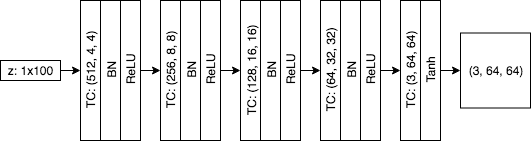
\includegraphics[scale=0.5]{network_structure}
  \caption{\gls{dcgan} Network Structure}
  \label{fig:network_structure}
\end{figure}

Figure \ref{fig:network_structure} shows the network structure of $G$, with five transposed convolutional
layers. Except for the last transposed convolutional layer, each of the previous four transposed convolutional
layers is followed by a layer of batch normalization, and a layer of \gls{relu} for
activation. Activation functions introduces nonlinearity to the network. The last transposed convolutional
layer is followed by a layer of $tanh$ function applied to each element as activation. The parameters for
each layer is detailed in Table \ref{table:network_layers}.  The network structure is rather simple,
compared with many other much larger networks. ResNet, for example, contains a deep cascade of 152 layers.

\begin{table}[h]
  \centering
  \caption{\gls{dcgan} Layers: TC stands for transposed convolution, BN stands for batch normalization}
  \begin{tabular}{l | l | l }
    \toprule
    Layer & Type & Description \\
    \midrule
    1 & TC & $100 \rightarrow 512$ channels, $4 \times 4$ kernel, stride $1$, padding $0$ \\
    2 & BN & $512$ channels\\
    3 & ReLU & $512$ channels \\
    4 & TC & $512 \rightarrow 256$ channels, $4 \times 4$ kernel, stride $2$, padding $1$ \\
    5 & BN & $256$ channels \\
    6 & ReLU & $256$ channels \\
    7 & TC & $256 \rightarrow 128$ channels, $4 \times 4$ kernel, stride $2$, padding $1$ \\
    8 & BN & $128$ channels \\
    9 & ReLU & $128$ channels \\
    10 & TC & $128 \rightarrow 64$ channels, $4 \times 4$ kernel, stride $2$, padding $1$ \\
    11 & BN & $64$ channels \\
    12 & ReLU & $64$ channels \\
    13 & TC & $64 \rightarrow 3$ channels, $4 \times 4$ kernel, stride $2$, padding $1$ \\
    14 & Tanh & 3 channels, final layer \\
    \bottomrule
  \end{tabular}
  \label{table:network_layers}
\end{table}

\section{Transposed Convolutional Layer}

In \gls{cnn}s, convolutional layer extracts various features from the input, essentially performing a
downsampling operation. Transposed convolutional layer, also known as fractionally strided convolutional
layers, or sometime erroneously as deconvolutional layer, on the other hand performs upsampling on the input.
Normally unsampling is often done with interpolation, but transposed convolution as a novel approach offers
trainability which makes it useful for neural networks. Conceptually, if a convolution layer of stride $f$
is run backwards, it can be seen as convolution layer with stride $1/f$, hence the name fractionally
strided convolution.

\subsection{Convolution}

To understand the operation of transposed convolution, it is perhaps natural to start with regular convolution
first. It is also helpful to work though a simple numerical example, starting with a $2D$ convolution
with an input of $4 \times 4$ matrix $A$:

$$
A =
  \begin{pmatrix}
    1 & 2 & 3 & 4 \\
    4 & 3 & 2 & 1 \\
    1 & 2 & 3 & 4 \\
    4 & 3 & 2 & 1
  \end{pmatrix}
$$

Let the kernel be a $2 \times 2$ matrix $K$:

$$
K =
  \begin{pmatrix}
    1 & 2 \\
    3 & 4
  \end{pmatrix}
$$

Assume the convolution operates with padding of $1$ and stride of $2$, that is, $K$ is slid across the
zero-padded matrix $B$ with a step of $2$, from left to right, top to bottom. $B$ is shown below:

$$
B =
  \begin{pmatrix}
    {\color{red}0} & {\color{red}0} & {\color{blue}0} & {\color{blue}0} & 0 & 0 \\
    {\color{red}0} & {\color{red}1} & {\color{blue}2} & {\color{blue}3} & 4 & 0 \\
    0 & 4 & 3 & 2 & 1 & 0 \\
    0 & 1 & 2 & 3 & 4 & 0 \\
    0 & 4 & 3 & 2 & 1 & 0 \\
    0 & 0 & 0 & 0 & 0 & 0
  \end{pmatrix}
$$

When $K$ is slid across $B$, the overlapping entries in $B$ is called a \textit{patch}. The first two
patches are shown in red and blue respectively. At each step, an element-wise inner product (Frobenius inner
product) $\langle K,P \rangle_{F}$ is computed between $K$ and the corresponding patch $P$ and stored as
an element in the result matrix $C$:

$$
C =
  \begin{pmatrix}
    4 & 8 & 12 \\
    12 & 25 & 13 \\
    8 & 7 & 1
  \end{pmatrix}
$$

In practice, the sliding-window approach is inefficient for implementation. All practical implementations
use a pair of operations called $im2col$ and $col2im$ to wrap a single matrix multiplication. Since
matrix multiplication is such a fundamental operation that its algorithm has been highly optimized over the
decades, and this vindicates the memory overhead caused by $im2col$. To start, flatten $K$ into a row vector
$K_{row}$:

$$
K_{row} =
  \begin{pmatrix}
    1 & 2 & 3 & 4 \\
  \end{pmatrix}
$$

For each patch in $B$ that $K$ convolves with, the entries in that patch are unrolled into a matrix $B_{col}$
made of column vectors:

$$
B_{col} =
  \begin{pmatrix}
    0 & 0 & 0 & 0 & 3 & 1 & 0 & 3 & 1 \\
    0 & 0 & 0 & 4 & 2 & 0 & 4 & 2 & 0 \\
    0 & 2 & 4 & 0 & 2 & 4 & 0 & 0 & 0 \\
    1 & 3 & 0 & 1 & 3 & 0 & 0 & 0 & 0
  \end{pmatrix}
$$

This operation is called $im2col$, namely, image to columns. Now, compute the product $K_{row} * B_{col}$, we
obtain a $1 \times 9$ matrix:

$$
\begin{pmatrix}
  4 & 18 & 12 & 12 & 25 & 13 & 8 & 7 & 1
\end{pmatrix}
$$

Finally this matrix is "reshaped" to the desired $3 \times 3$ output which is $C$ using the operation $col2im$.

\subsection{Represent Convolution as a Sparse Matrix}

The procedure described in the previous section is how regular convolution would be implemented in practice.
On the other hand, there is an alternative view of the convolution, also performed with a single
matrix multiplication. This alternative view is impractical for implementation, but from which
input and output can be easily reversed. To see this, first unroll the zero-padded input $B$ into
a $36 \times 1$ matrix:

\setcounter{MaxMatrixCols}{20}

$$
B'^\intercal =
  \begin{pmatrix}
    0 & 0 & 0 & 0 & 0 & 0 & 0 & 1 & 2 & 3 & 4 & 0 & 0 & 4 & \dots
  \end{pmatrix}
$$

The output $C$ is also unrolled into a $9 \times 1$ matrix:

$$
C'^\intercal =
  \begin{pmatrix}
    4 & 18 & 12 & 12 & 25 & 13 & 8 & 7 & 1
  \end{pmatrix}
$$

Then the convolution can be represented as a sparse matrix $M$ of $9 \times 36$ with entries from kernel $K$,
one patch per row:

$$
M =
  \begin{pmatrix}
    1 & 2 & 0 & 0 & 0 & 0 & 3 & 4 & 0 & 0 & 0 & 0 & \dots \\
    0 & 0 & 1 & 2 & 0 & 0 & 0 & 0 & 3 & 4 & 0 & 0 & \dots \\
    \vdots \\
  \end{pmatrix}
$$

$M$ takes $B'$ as input and produces $C'$ as output, which again can be reshaped to $C$.

\subsection{Transposed Convolution}

In the previous section, the convolution is represented as a kernel-defined sparse matrix. Under this view,
it is very easy to derive the \textit{backward pass}. This example convolution maps an input of $4 \times 4$
to an output of $3 \times 3$, to reverse the direction of input and output, namely, to take an input of
$3 \times 3$ and produce an output of $4 \times 4$, all it takes is to transpose $M$ to obtain $M^\intercal$
of $36 \times 9$. When $M^\intercal$ is applied to the an $3 \times 3$ input unrolled to $9 \times 1$, the
resulting $36 \times 1$ matrix is then reshaped to the desired $4 \times 4$ output. Hence the name
\textit{transposed convolution}.

It needs to be pointed out that the term \textit{backward pass} instead of \textit{inverse operation},
since $M^\intercal$ does not recover the numerical values of $B$ from $C$, it only recovers the shape of $B$,
therefore it is misleading to call this operation deconvolution.

\section{Batch Normalization Layer}

Batch normalization is an operation defined as

\begin{equation} \label{eq:batch_normalization}
  y = \gamma \frac{x - \bar{x}}{\sqrt{\sigma^2(x) + {eps}}} + \beta
\end{equation}

Here $eps$ is a small constant that adds to numerical stability. $\gamma$ and $\beta$ can be regarded
as trained weight and bias. The output $y$ of the normalization would have a mean of zero and standard
deviation of one. Batch normalization optimizes the training of the network, making it converge
faster with higher learning rates. It can also improve overall accuracy of the model. For deep networks
like \gls{dcgan}, it is a key ingredient.

However, this operation involves an inversed square root operation $\frac{1}{\sqrt{\sigma^2(x) + eps}}$,
which is rather difficult to compute with fixed-point numbers. Luckily Xilinx Vivado includes an IP which
can both convert between fixed-point and floating-point representations, as well as compute inversed square
root.

\section{Activation Layer}

Activation function, also known as \textit{transfer function}, adds non-linearity to the network. It is often
attached to the output of a layer, typically mapping the results to the range $(0, 1)$ or $(-1, 1)$, although
other possibilities exist. Assume the functions maps the input to range $(0, 1)$, a value close to $0$ would
be seen as "off" or "no", a value close to $1$ would be seen as "on" or "yes". This indicates whether the
following connection should see this output as activated or not, hence the name activation function.

Many different types of activation functions exist with two main categories: linear and nonlinear. A commonly
used sigmoid (S-shaped) function is $y = \frac{1}{1 + e^{-x}}$, shown in \ref{fig:sigmoid_relu}.

\begin{figure}[h]
  \centering
  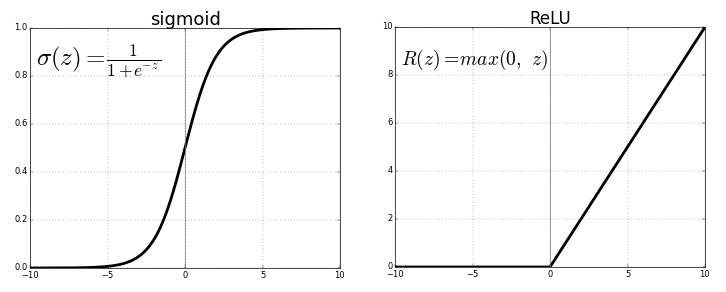
\includegraphics[scale=0.5]{sigmoid_relu}
  \caption{Sigmoid vs. ReLU}
  \label{fig:sigmoid_relu}
\end{figure}

\subsection{ReLU Layer}

ReLU is very popular nowadays. It is defined as

\begin{equation} \label{eq:relu}
  y = max(0, x)
\end{equation}

The first thing to notice is that it is in fact nonlinear. When compared with the sigmoid function, the
gradient of ReLU does not saturate when $x$ gets large, which makes \gls{sgd} convergence faster. In addition,
since all negative values are converted to zero, it adds the desirable feature of sparsity to the network,
making computation efficient. The implementation of ReLU is of course straightforward.

\subsection{Tanh Layer}

The hyperbolic tangent function $tanh$ is another widely used activation function. It works similarly to the
sigmoid function with the additional property of being symmetrical with respect to the origin.

\begin{equation} \label{eq:tanh}
  \begin{split}
    y & = \frac{e^x - e^{-x}}{e^{x} + e^{-x}} \\
      & = \frac{e^{2x} - 1}{e^{2x} + 1} \\
      & = \frac{1- e^{-2x}}{1 - e^{-2x}}
  \end{split}
\end{equation}

\begin{figure}[h]
  \centering
  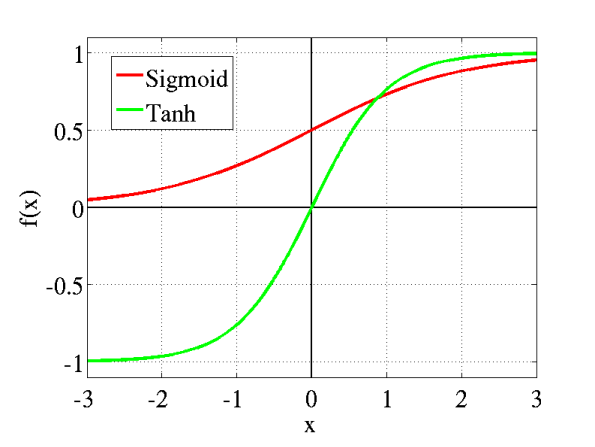
\includegraphics[scale=0.5]{sigmoid_tanh}
  \caption{Sigmoid vs. Tanh}
  \label{fig:sigmoid_tanh}
\end{figure}

\clearpage %force the next chapter to start on a new page. Keep that as the last line of your chapter!

% Project Specifications

\chapter{Generator Layers}

\section{Transposed Convolutional Layer}

In CNNs, convolutional layer extracts various features from the input, essentially performing a downsampling
operation. Transposed convolutional layer, also known as fractionally strided convolutional layers, or sometime
erroneously as deconvolutional layer, on the other hand performs upsampling on the input. Normally unsampling
is often done with interpolation, but transposed convolution as a novel approach offers trainability which
makes it useful for neural networks. Conceptually, if we run a convolution of stride $f$ backwards,
it can be seen as convolution with stride $1/f$, hence the name fractionally strided convolution.

\subsection{Convolution}

To understand its operation, let us work though a simple numerical example. We begin with regular convolution
with an input of $4 \times 4$ matrix $A$:

$$
A =
  \begin{pmatrix}
    1 & 2 & 3 & 4 \\
    4 & 3 & 2 & 1 \\
    1 & 2 & 3 & 4 \\
    4 & 3 & 2 & 1
  \end{pmatrix}
$$

Let the kernel be a $2x2$ matrix $K$:

$$
K =
  \begin{pmatrix}
    1 & 2 \\
    3 & 4
  \end{pmatrix}
$$

Assume the convolution operates with padding of $1$ and stride of $2$, that is, we slide $K$ across the
zero-padded matrix $B$ with a step of $2$. $B$ is shown below:

$$
B =
  \begin{pmatrix}
    0 & 0 & 0 & 0 & 0 & 0 \\
    0 & 1 & 2 & 3 & 4 & 0 \\
    0 & 4 & 3 & 2 & 1 & 0 \\
    0 & 1 & 2 & 3 & 4 & 0 \\
    0 & 4 & 3 & 2 & 1 & 0 \\
    0 & 0 & 0 & 0 & 0 & 0
  \end{pmatrix}
$$

When $K$ is slided across $B$, the overlapping entries in $B$ is called a \textit{patch}. If we view $K$ and
the corresponding patch in $B$ as vectors, at each step, a dot product is computed between them and stored as
an element in the result matrix $C$:

$$
C =
  \begin{pmatrix}
    4 & 8 & 12 \\
    12 & 25 & 13 \\
    8 & 7 & 1
  \end{pmatrix}
$$

In practice, the sliding-window approach is inefficient for implementation. All practical implementations
use a pair of operations called $im2col$ and $col2im$ to wrap a single matrix multiplication. Since
matrix multiplication is such a fundamental operation that its algorithm has been highly optimized over the
decades, and this vindicates the memory overhead caused by $im2col$. To start, flatten $K$ into a row vector
$K_{row}$:

$$
K_{row} =
  \begin{pmatrix}
    1 & 2 & 3 & 4 \\
  \end{pmatrix}
$$

For each patch in $B$ that $K$ convolves with, the entries in that patch are unrolled into a matrix $B_{col}$
made of column vectors:

$$
B_{col} =
  \begin{pmatrix}
    0 & 0 & 0 & 0 & 3 & 1 & 0 & 3 & 1 \\
    0 & 0 & 0 & 4 & 2 & 0 & 4 & 2 & 0 \\
    0 & 2 & 4 & 0 & 2 & 4 & 0 & 0 & 0 \\
    1 & 3 & 0 & 1 & 3 & 0 & 0 & 0 & 0
  \end{pmatrix}
$$

This operation is called $im2col$, namely, image to columns. Now, compute the product $K_{row} * B_{col}$, we
obtain a $1x9$ matrix:

$$
\begin{pmatrix}
  4 & 18 & 12 & 12 & 25 & 13 & 8 & 7 & 1
\end{pmatrix}
$$

Finally we "reshape" this matrix to the desired $3 \times 3$ output which is $C$ using the operation $col2im$.

\subsection{Represent Convolution as a Sparse Matrix}

Recall that the precedure described above is how regular convolution would be implemented in practice.
On the other hand, there exists an alternative view of the convolution, also performed with a single
matrix multiplication. This alternative view is impractical for implementation, but from which
we can easily reverse the input and output. To see this, first unroll the zero-padded input $B$ into
a $36 \times 1$ matrix:

\setcounter{MaxMatrixCols}{20}

$$
B'^\intercal =
  \begin{pmatrix}
    0 & 0 & 0 & 0 & 0 & 0 & 0 & 1 & 2 & 3 & 4 & 0 & 0 & 4 & \dots
  \end{pmatrix}
$$

The output $C$ is also unrolled into a $9 \times 1$ matrix:

$$
C'^\intercal =
  \begin{pmatrix}
    4 & 18 & 12 & 12 & 25 & 13 & 8 & 7 & 1
  \end{pmatrix}
$$

Then the convolution can be represented as a sparse matrix $M$ of $9 \times 36$ with entries from kernel $K$,
one patch per row:

$$
M =
  \begin{pmatrix}
    1 & 2 & 0 & 0 & 0 & 0 & 3 & 4 & 0 & 0 & 0 & 0 & \dots \\
    0 & 0 & 1 & 2 & 0 & 0 & 0 & 0 & 3 & 4 & 0 & 0 & \dots \\
    \vdots \\
  \end{pmatrix}
$$

$M$ takes $B'$ as input and produces $C'$ as output, which again can be reshaped to $C$.

\subsection{Transposed Convolution}
In the previous section, the convolution is represented as a kernel-defined sparse matrix. Under this view,
it is very easy to derive the \textit{backward pass}. This example convolution maps an input of $4 \times 4$
to an output of $3 \times 3$, to reverse the direction of input and output, namely, to take an input of
$3 \times 3$ and produce an output of $4 \times 4$, all it takes is to transpose $M$ to obtain $M^\intercal$
of $36 \times 9$. When $M^\intercal$ is applied to the an $3 \times 3$ input unrolled to $9 \times 1$, the
resulting $36 \times 1$ matrix is then reshaped to the desired $4 \times 4$ output. Hence the name
\textit{transposed convolution}.

Notice that we use the term \textit{backward pass} instead of \textit{inverse operation}, since $M^\intercal$
does not recover the numerical values of $B$ from $C$, it only recovers the shape of $B$. And that is why it
is misleading to call this operation deconvolution.

\section{Batch Normalization Layer}

Batch normalization is an operation defined as

\begin{equation} \label{eq:batch_normalization}
  y = \gamma \frac{x - \bar{x}}{\sqrt{\sigma^2(x) + {eps}}} \gamma + \beta
\end{equation}

Here $eps$ is a small constant that adds to numerical stability. $\gamma$ and $\beta$ can be regarded
as trained weight and bias. The output $y$ of the normalization would have a mean of zero and standard
deviation of one. Batch normalization optimizes the training of the network, making it converge
faster with higher learning rates. It can also improve overall accuracy of the model. It is a key ingredient
for deep networks such as DSGANs.

However, this operation involves an inversed square root operation $\frac{1}{\sqrt{\sigma^2(x) + eps}}$,
which is rather difficult to compute with fixed-point numbers. Luckily Xilinx Vivado includes an IP which
can both convert between fixed-point and floating-point representations, as well as compute inversed square
root.

\section{Activation Layer}

Activation function, also known as \textit{transfer function}, adds non-linearity to the network. It is often
attached to the output of a layer, typically mapping the results to the range $(0, 1)$ or $(-1, 1)$, although
other possibilities exist. Assume the functions maps the input to range $(0, 1)$, a value close to $0$ would
be seen as "off" or "no", a value close to $1$ would be seen as "on" or "yes". This indicates wheather the
following connection should see this output as activated or not, hence the name activation function.

Many different types of activation functions exist with two main categories: linear and non-lear. A commonly
used sigmoid (S-shaped) function is $y = \frac{1}{1 + e^(-x)}$, shown in \ref{fig:sigmoid_relu}.

\begin{figure}[h]
  \centering
  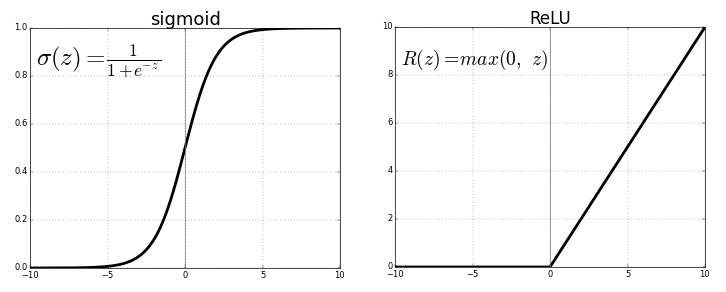
\includegraphics[scale=0.5]{sigmoid_relu}
  \caption{Sigmoid vs. ReLU}
  \label{fig:sigmoid_relu}
\end{figure}

\subsection{ReLU Layer}

ReLU is very popular nowadays. It is defined as

\begin{equation} \label{eq:relu}
  y = max(0, x)
\end{equation}

When compared with the sigmoid function, the gradient of ReLU does not saturate when $x$ gets large,
which makes SGD convergence faster. In addition, since all negative values are converted to zero, it adds
the desirable feature of sparsity to the network, making computation efficient. The implementation of ReLU
is of course straightforward.

\subsection{Tanh Layer}

The hyperbolic tangent function $tanh$ is another widely used activation function. It works similarly to the
sigmoid functon with the additional property of being symmetrical with respect to the origin.

\begin{equation} \label{eq:tanh}
  \begin{split}
    y & = \frac{e^x - e^{-x}}{e^{x} + e^{-x}} \\
      & = \frac{e^{2x} - 1}{e^{2x} + 1} \\
      & = \frac{1- e^{-2x}}{1 - e^{-2x}}
  \end{split}
\end{equation}

\begin{figure}[h]
  \centering
  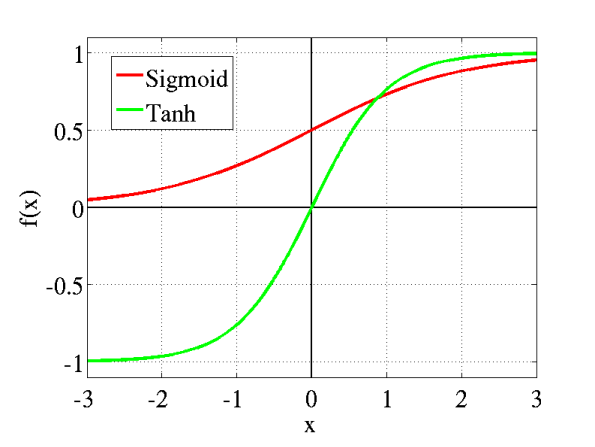
\includegraphics[scale=0.5]{sigmoid_tanh}
  \caption{Sigmoid vs. Tanh}
  \label{fig:sigmoid_tanh}
\end{figure}

\clearpage %force the next chapter to start on a new page. Keep that as the last line of your chapter!

% Project Specifications

\chapter{GEMM and $col2im$}

The previous chapter discussed different ways to view the convolution operation and its cousin,
the transposed convolution, both conceptually and implementationally. When it comes down to implementation,
we have seen that both operations can be implemented with a single matrix multiplication. In other words,
matrix multiplication is the main computational burden of these operations. Meanwhile, real world applications
often involve very large matrices. Therefore, as a low-level operation, the implementation of matrix
multiplication is often heavily optimized.

\gls{gemm} is considered as the \textit{de facto} standard operation
contained in the \gls{blas} specification. It has many implementations for
different platforms which exhaustively utilize various optimizations like \gls{simd} instructions,
parallelism, cache-awareness, etc.

\gls{gemm} is defined as

$$C \leftarrow \alpha op(A) op(B) + \beta C,$$

where $\alpha, \beta \in \mathbb{R}$, $op(X)$ is either $X$ or $X^\intercal$. In our particular case for
transposed convolution, $\alpha = 1$, $\beta = 0$, $op(X) = X$, so \gls{gemm} reduces to the basic
matrix multiplication $C \leftarrow A B$.

A subtle detail in the implementation of \gls{gemm} is the order of storage of matrix entries. There are two
different orders to store the same matrix: row-major order or column-major order. In row-major order,
entries of rows are stored contiguously in memory, while in column-major order, entries of columns are
consecutive to each other in memory.

A naïve implementation of \gls{gemm} is shown in Listing \ref{code:naivegemm}. Here,
\mintinline{c}{lda}, \mintinline{c}{ldb} and \mintinline{c}{ldc} are
leading dimension of matrix $A$, $B$ and $C$, respectively.

\begin{code}
\begin{minted}{c}
for (int i = 0; i < m; i++) {
    for (int j = 0; j < n; j++) {
        float sum = 0;
        for (int l = 0; l < k; l++)
          sum += a[l*lda+i] * b[l*ldb+j];
        c[j*ldc+i] = beta * c[j*ldc+i] + alpha * sum;
    }
}
\end{minted}
  \captionof{listing}{Naïve C Implementation of \gls{gemm}}
\label{code:naivegemm}
\end{code}

This implementation is straightforward and not very efficient, but it is a good starting point to guide
us through the rest of the design.

Another operation used by transposed convolution is $col2im$. It cherry picks the elements computed by
\gls{gemm} and places them in the destination image. To describe $col2im$, it is necessary to introduce
the variables used for transposed convolution.

\begin{itemize}
  \item \mintinline{c}{inputHeight} and \mintinline{c}{inputWidth} are the height and width of each input
    channel (sometimes also called input plane)
  \item \mintinline{c}{nInputChannel} is the number of input channel in total, thus the input is a
    $3D$ tensor with dimensions \mintinline{c}{(nInputChannel, inputHeight, inputWidth)}
  \item With \mintinline{c}{m = inputHeight * inputWidth} and \mintinline{c}{k = nInputChannel}, the input
    tensor is stored as a matrix $A \in \mathbb{R}^{m \times k}$
  \item \mintinline{c}{kernelH} and \mintinline{c}{kernelW} are the height and width of each
    convolutional kernel channel
  \item Each kernel is also a $3D$ tensor with dimensions \mintinline{c}{(nInputChannel, kernelH, kernelW)}
  \item \mintinline{c}{nOutputChannel} is the number of output channels
  \item There are \mintinline{c}{nOutputChannel}'s of kernels, each responsible for producing an output channel
  \item With \mintinline{c}{k = nInputChannel} and \mintinline{c}{n = nOutputChannel * kernelH * kernelW},
    the kernel tensor is stored as a matrix $B \in \mathbb{R}^{k \times n}$
\end{itemize}

The code of $col2im$ is given in listing \ref{code:col2im}:

\begin{code}
\begin{minted}{c}
// content of data_im set to 0 already
const int n = nOutputChannel * kernelH * kernelW;
for (int j = 0; j < n; ++j) {
    int w_offset = j % kernelW;
    int h_offset = (j / kernelW) % kernelH;
    int c_im = j / kernelH / kernelW;
    for (int h_col = 0; h_col < inputHeight; ++h_col) {
        for (int w_col = 0; w_col < inputWidth; ++w_col) {
            int h_im = h_col * strideH - padH + h_offset * dilationH;
            int w_im = w_col * strideW - padW + w_offset * dilationW;
            if (h_im >= 0 && h_im < outputHeight &&
                w_im >= 0 && w_im < outputWidth) {
                data_im[(c_im * outputHeight + h_im) * outputWidth + w_im] +=
                    data_col[(j * inputHeight + h_col) * inputWidth + w_col];
            }
        }
    }
}
\end{minted}
\captionof{listing}{C Implementation of $col2im$}
\label{code:col2im}
\end{code}

Here \mintinline{c}{data_im} is the target image while \mintinline{c}{data_col} is the result of \gls{gemm}.
The outermost loop iterates through the columns of $C \in \mathbb{R}^{k \times n}$. The two nested loops
iterate the rows of $C$, since \mintinline{c}{m = inputHeight * inputWidth}. \mintinline{c}{c_im} is the
index of the channel in the output image. %\mintinline{c}{h_offset} and \mintinline{c}{w_offset} are the offset in each 

For transposed convolution, \mintinline{c}{data_im} is typically smaller than
\mintinline{c}{data_col}. This leads to a key optimization idea: it is possible to merge \gls{gemm} and
$col2im$ together and compute transposed convolution by doing \gls{gemm} sparsely. In doing so,
\mintinline{c}{data_col} can be abandoned and the results will be directly placed in \mintinline{c}{data_im},
that is, there is no need for an extra large buffer for intermediate results.

\begin{code}
\begin{minted}{c}
int j = 0;
for (int c_im = 0; c_im < nOutputChannel; c_im++) {
    for (int h_offset = 0; h_offset < kernelH; h_offset++) {
        for (int w_offset = 0; w_offset < kernelW; w_offset++) {
            int i = 0;
            for (long h_col = 0; h_col < inputHeight; h_col++) {
                for (long w_col = 0; w_col < inputWidth; w_col++) {
                    int h_im = h_col * strideH - padH + h_offset * dilationH;
                    int w_im = w_col * strideW - padW + w_offset * dilationW;
                    if (h_im >= 0 && h_im < outputHeight &&
                        w_im >= 0 && w_im < outputWidth) {
                        float sum = 0;
                        for (long l = 0; l < k; l++)
                            sum += a[l*lda + i] * b[l*ldb + j];
                        int idx = (c_im * outputHeight + h_im) *
                                  outputWidth + w_im;
                        data_im[idx] += sum;
                    }
                    i++;
                }
            }
            j++;
        }
    }
}
\end{minted}
\captionof{listing}{C Implementation of $transposed\_convolution$}
\label{code:transposed_convolution_in_c}
\end{code}

The key to understand this code of merge is to notice that the for-loop indexed by \mintinline{c}{j} in
\mintinline{c}{gemm} can be splitted into three nested for-loop indexed by \mintinline{c}{c_im},
\mintinline{c}{h_offset} and \mintinline{c}{w_offset}.
Similarly, the for-loop indexed by \mintinline{c}{i} in \mintinline{c}{gemm} is equivalent to the two
nested for-loop indexed by \mintinline{c}{h_col} and \mintinline{c}{w_col}, same as in \mintinline{c}{col2im}.

This last C code in listing \ref{code:transposed_convolution_in_c} serves as the blueprint for implementing
transposed convolution on \gls{fpga} with Verilog.

\clearpage %force the next chapter to start on a new page. Keep that as the last line of your chapter!

% Project Specifications

\chapter{Quantization}

%In such networks a large part of the computation is done with an
%operation called the \gls{gemm}. An efficient implementation of \gls{gemm} is crucial to the
%acceleration. However, \glspl{cnn} are normally implemented with floating-point numbers, which are usually less
%efficient to handle in hardware than fixed-point numbers. A class of techniques called quantization can
%be used to carry out the computation in fixed-point numbers and then convert the result back to
%floating-point numbers, realizing high performance in hardware. Chapter 4 provides a detailed discussion
%of the quantization scheme used in this project.

Machine learning programs normally represent numbers as floating-point. Although floating-point numbers
have limited precision and can sometimes lead to numerical instability when the numbers involved get too
small or too large, they are intuitive and easy to work with. But floating-point arithmetic can be rather
expensive to implement in hardware. Modern \glspl{fpga} contain dedicated \gls{dsp} unit, some of which
natively
support floating-point, others require special \gls{ip} cores to implement the relevant
circuitry. \gls{fpga}'s processing power mainly shines on fixed-point. In order to run our model in fixed-point
on \gls{fpga}, it is necessary to convert the model into fixed-point representation, through a process known as
quantization. When the result is computed by \gls{fpga}, it is then converted back to floating-point, which is
naturally called dequantization.

Quantization brings additional benefits with the compression of model size. When 32-bit floating-point
numbers are quantized to 8-bit, the model size is reduced by $75\%$. This cuts down memory bandwidth
requirement and improves memory efficiency. Consequently, the power consumption can be greatly reduced.

One could imagine that quantization would cause a tremendous loss to model precision, for example, when
32-bit floating-point numbers (ranging from $1.175494351 \times 10^{-38}$ to $3.402823466 \times 10^38$) are converted to
8-bit unsigned integers (ranging from 0 to 255). However, one of the peculiar
properties of neural networks is that they are very resilient to noise. Of course this is also one of the
reasons why they are so successful in real world applications. We could view the internal precision loss of
quantization as a form of internal noise, it turned out that the precision loss incurred is rather small.

There exist many different quantization methods. This project adopted the quantization scheme
implemented in Google's \textit{gemmlowp} library, a low precision GEMM implementation for fixed-point. The
original 32-bit single-precision weights represented in $float$ are mapped to $uint8\_t$. GEMM is then
carried out on the \gls{fpga} board with these 8-bit integers. Intermediate MACC results are 32-bit
integers to accommodate the accumulation. Eventually the final output of the model is converted back to
$float$.

The quantization works by first identifying the range of the data. In neural networks, the values are usually
distributed within a relatively small range. For instance, for 8-bit quantization, if the minimum of the
weights is $-10.0$ and maximum is $20.0$, then $-10.0$ would be mapped to $0$, and $20.0$ mapped to $255$.
However, there is an additional requirement that can bring great benefits to subsequent computations:
the real value $0$ should be exactly representable. As will be shown, this can be achieved with a small
modification to the mapping equation.

Th quantization scheme can be derived with basic algebra. Define a real number $f$ as the result of an affine
mapping $f = S q + B$, where $q$ is the corresponding quantized integer, $S \in \mathbb{R}$ is a constant
scaling factor, and $B \in \mathbb{R}$ is a constant shift. Next, modify the mapping a bit so that the
real value $0$ is exactly representable:

\begin{equation} \label{eq:dequantization}
  f = S(q - Z),
\end{equation}

where $Z \in \mathbb{N}$ is a constant shift applied to $q$. Since convolution and transposed convolution
both can involve zero-padding, having an exact representation of $0$ avoids the accumulation of errors
(essentially a form of bias). With this form of affine mapping, $0$ is trivially mapped to $q = Z$. $S$ and
$Z$ are called the quantization parameters of this mapping. From equation \ref{eq:dequantization},
it is clear the quantization mapping is done with

\begin{equation} \label{eq:quantization}
  q = \frac{f}{S} + Z
\end{equation}

Let $A \in \mathbb{R}^{m \times k}$, $B \in \mathbb{R}^{k \times n}$, $A B = C \in \mathbb{R}^{m \times n}$,
the corresponding quantization parameters for $A$, $B$ and $C$ are $S_A$ and $Z_A$, $S_B$ and $Z_B$,
$S_C$ and $Z_C$. These parameters are predetermined, since in most cases the range of numbers in these matrices
are known. Let $p$, $q$, $r$ be the entries in the quantized version of $A$, $B$ and $C$. 

For an entry $f_C$ in $C$, $f_C = \sum_{i}^{} A_i B_i$, where $i$ is the index of entries in a particular
row in $A$ and corresponding column in $B$,

\begin{equation}
\begin{split}
  f_C & = \sum_{i} A_i B_i \\
      & = \sum_{i} S_A (p_i - Z_A) S_B (q_i - Z_A) \\
      & = S_A S_B \sum_{i} (p_i - Z_A) (q_i - Z_B)
\end{split}
\end{equation}

Clearly the term $\sum_{i} (p_i - Z_A) (q_i - Z_B)$ is the computational core here, let it be
$\mathfrak{K}$. We have

\begin{equation}
\begin{split}
  r_C & = \frac{f_C}{S_C} + Z_C \\
      & = \frac{S_A S_B}{S_C} \mathfrak{K} + Z_C
\end{split}
\end{equation}

Therefore, once $\mathfrak{K}$ is computed, we can simply multiply it by a constant multiplier
$M = \frac{S_A S_B}{S_C}$, then add the zero offset $Z_C$ to obtain the quantized value $r_C$. The computation
of $\mathfrak{K}$ might seem problematic at first: it contains a subtraction operation for each entry,
which would bring extra overhead to the GEMM computation. Let us expand this expression:

\begin{equation}
\begin{split}
  \mathfrak{K} & = \sum_{i} (p_i - Z_A) (q_i - Z_B) \\
               & = \sum_{i} (p_i q_i - Z_B p_i - Z_A q_i + Z_A Z_B) \\
               & = \sum_{i} p_i q_i - \sum_{i} Z_B p_i - \sum_{i} Z_A q_i + \sum_{i} Z_A Z_B \\
               & = \sum_{i} p_i q_i - Z_B \sum_{i} p_i - Z_A \sum_{i} q_i + k Z_A Z_B
\end{split}
\end{equation}

Note that $\sum_{i} 1$ is k, the number of columns of $A$ and the number of rows of $B$. We have obtained
four terms here. The first term $\sum_{i} p_i q_i$ is the main term. The second term, $- Z_B \sum{i} p_i$
is the product of $- Z_B$ and the sum of the current row, which only needs to be calculated once and added
to each result of the first term. The third term $- Z_A \sum{i} q_i$ and the fourth term $k Z_A Z_B$ are
similar. The computation can be carried out by computing the first term as the core, and add the rest three
terms one by one.

\section{Handling of Bias}

Biases are added to the 32-bit accumulator result. Recall that $f_C = \sum_{i} A_i B_i = S_A S_B \mathfrak{K}$,
it is clear that biases should be quantized with $S = S_A S_B$ and $Z = 0$. When zero offset is $0$, negative
numbers will remain negative, consequently the type of bias values should be signed 32-bit integers.

\clearpage %force the next chapter to start on a new page. Keep that as the last line of your chapter!

% Project Specifications

\chapter{Hardware Architecture}

\section{Hardware Resources}

The development board for this project is Nexys 4 from Digilent with an Artix-7 \gls{fpga} chip from Xilinx.
Table \ref{table:hardware_resources} summarizes the hardware resources available on the Nexys 4 board.

% [h] means here, can use [h!] to override internal LaTeX parameters
\begin{table}[h]
  \centering
  \caption{Nexys 4 Resource Specifications}
  \begin{tabular}{l | l}
    Logic Slices & 15850 \\
    Block RAM & 4860 Kbits \\
    DSP Slices & 240 \\
    Cellular RAM & 16MB \\
    Quad-SPI Flash & 16MB
  \end{tabular}
  \label{table:hardware_resources}
\end{table}

\section{Calculate Memory Requirement}

\gls{bram} will be the main active memory for input, output, weight, and bias data. The \gls{fpga} chip in use
contains 4860 Kbits of \gls{bram}, which is 607.5KB. The original model size is around 13.7MB, which is
considered very compact when compared with other deep learning models but still very demanding for
our system. Once quantized, the model size is roughly 3.5MB. So it is not possible to fit the entire model
into the \gls{bram} and it is inevitable to interact with external storage devices, e.g., the 16MB Quad-SPI
Flash or the 16MB \gls{psram} on the Nexys 4 board.

Because the resources on the board is quite limited, it is easiest to compute the model in a layer-by-layer
fashion without exploiting the layer-wise parallelism. First, the weights of a transposed
convolutional layer are read from the external storage device, the layer is then computed, followed by one or
more auxiliary layers such as batch normalization or activation layer. The output is then transfered from
the output \gls{bram} buffer to the input \gls{bram} buffer, then the weights of the next transposed
convolutional layer are read and the process continues until it reaches the final layer.

In order to allocate \gls{bram} properly, it is necessary to list the detailed memory requirements of each
layer.

\begin{table}[h]
  \centering
  \caption{Memory Requirement by Layers}
  \begin{tabular}{l | l | l | l | l}
    \toprule
    Layer & Input & Weight & Bias & Output \\
    \midrule
    1 & 100(8) & 819200(8) & 512(32) & 8192(32) \\
    2 & 8192(32) & 512(32) & 512(32) & 8192(32) \\
    3 & 8192(32) & - & - & 8192(8) \\
    4 & 8192(8) & 2097152(8) & 256(32) & 16384(32) \\
    5 & 16384(32) & 256(32) & 256(32) & 16384(32) \\
    6 & 16384(32) & - & - & 16384(8) \\
    7 & 16384(8) & 524288(8) & 128(32) & 32768(32) \\
    8 & 32768(32) & 128(32) & 128(32) & 32768(32) \\
    9 & 32768(32) & - & - & 32768(8) \\
    10 & 32768(8) & 131072(8) & 64(32) & 65536(32) \\
    11 & 65536(32) & 64(32) & 64(32) & 65536(32) \\
    12 & 65536(32) & - & - & 65536(8) \\
    13 & 65536(8) & 3072(8) & 3(32) & 12288(32) \\
    14 & 12288(32) & - & - & 12288(8) \\
    \bottomrule
  \end{tabular}
  \label{table:memory_requirements}
\end{table}

In table \ref{table:memory_requirements}, the numbers in parentheses are the bit width of the values. The table
indicates the maximum input/output size is 65536 in 32-bit, the maximum weight size is 2097152 in 8-bit, the
maximum bias size is 512 in 32-bit. However, notice that when both input is 65536 in 32-bit, the corresponding
layers are batch normalization and ReLU. This means that the same buffer can be used to store both the
input and output because the input can be updated in-place. Consequently the input buffer only needs to
store 65536 values in 8-bit.

To conclude, four main buffers are needed: input buffer (65536 bytes), output buffer (262144 bytes),
weight buffer (2097152 bytes), bias buffer (16384 bytes). Some auxiliary buffers are needed to store
the quantization parameters.

\section{Architecture}

The system stores weights of transposed convolutional layer in the 16MB Quad-SPI Flash. A computation unit
contains a transposed convolution module TC, a batch normalization module BN, a ReLU module ReLU,
and a tanh module Tanh. The unit can be configured to be TC-BN-ReLU or TC-Tanh. The network computes one
layer at a time. Before reading the final layer, the output of the computation unit is transferred to the
input buffer. The final result is sent to computer via \gls{uart} (serial port). Figure
\ref{fig:computation_unit} shows the structure of the computation unit.

\begin{figure}[h]
  \centering
  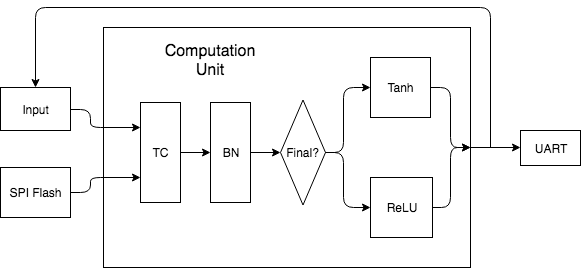
\includegraphics[scale=0.75]{computation_unit}
  \caption{Computation Unit Block Diagram}
  \label{fig:computation_unit}
\end{figure}

The input of the TC module are quantized 8-bit integers, while the output of the TC module are 32-bit
integers, which are input to the BN module. The BN first dequantizes the 32-bit input to 32-bit
single-precision floating-point numbers according to IEEE 754 standard, then the computation is carried
out in floating-point and the results are fed to the ReLU module, which simply sets negative values to
$0.0$ and then quantizes the output to 8-bit integers again and overwrites the input buffer with the
results. When the flow reaches the final Tanh module, the 32-bit input integers are dequantized just as the
BN module, $tanh$ is then performed on the floating-point numbers, and the final floating-point result is
sent to the computer through \gls{uart}, which can then be displayed with a simple conversion script.

\clearpage %force the next chapter to start on a new page. Keep that as the last line of your chapter!

% Project Specifications

\chapter{Implementation Details}

\section{Development Environment and Method}

Xilinx Vivado version 2017.04 is used as the development platform for FPGA. The typical workflow involves
the following steps: design the functionality of module, implement the module in Verilog, add IP blocks
if necessary, write the testbench for the module, run behavioral simulation, run synthesis and implementation,
run post-synthesis and post-implementation simulation, view synthesis and implementation reports, and finally,
create bitstream and test on device.

A parallel C implementation is developed on Linux simultaneously to facilitate the FPGA development.
Its main function is to provide algorithm verification, especially numerical comparison of output layers
between software implementation and FPGA implementation.

\section{Implementing the Transposed Convolutional Layer}

The DSP48 Macro IP is utilized to accomplish computations with multiplication and accumulation. The first
block implements the operations shown in \ref{table:dsp48_0_operations}. The second block is the core MACC
unit, and only contains $P \leftarrow A*B+P$.

\begin{table}[h]
  \centering
  \caption{DSP48 #0 Operations}
  \begin{tabular}{l | l}
    0 & $P \leftarrow A*B-C$ \\
    1 & $P \leftarrow A*B+PCIN$ \\
    2 & $P \leftarrow A*B+C$
  \end{tabular}
  \label{table:dsp48_0_operations}
\end{table}

The ports of both blocks are shown in \ref{fig:dsp48_macro_0} and \ref{fig:dsp48_macro_1}.

\begin{figure}[h]
  \centering
  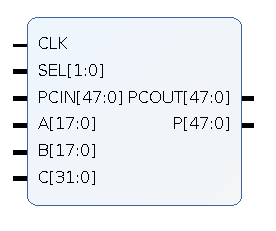
\includegraphics[scale=0.5]{dsp48_macro_0}
  \caption{DSP48 Macro #0 Ports}
  \label{fig:dsp48_macro_0}
\end{figure}

\begin{figure}[h]
  \centering
  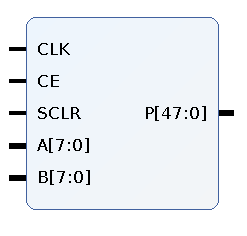
\includegraphics[scale=0.5]{dsp48_macro_1}
  \caption{DSP48 Macro #1 (MACC) Ports}
  \label{fig:dsp48_macro_1}
\end{figure}

\subsection{DSP48 Pipelining}

The DSP48 slice can be used without pipelining. However, that is essentially a combinational circuit and
the propagation delay will significantly reduce $F_{max}$. To run the FPGA at a higher frequency, it is
necessary to use pipeline registers. In our first design, only the register after the multiplier is used
therefore the result is delayed by one clock cycle.

\begin{figure}[h]
  \centering
  \includegraphics[scale=0.5]{dsp48_macro_1_pipeline}
  \caption{DSP48 Macro #0 Pipeline Configuration}
  \label{fig:dsp48_macro_1_pipeline}
\end{figure}

\clearpage %force the next chapter to start on a new page. Keep that as the last line of your chapter!

% Project Specifications

\chapter{Testbench}

\begin{figure}[h]
  \centering
  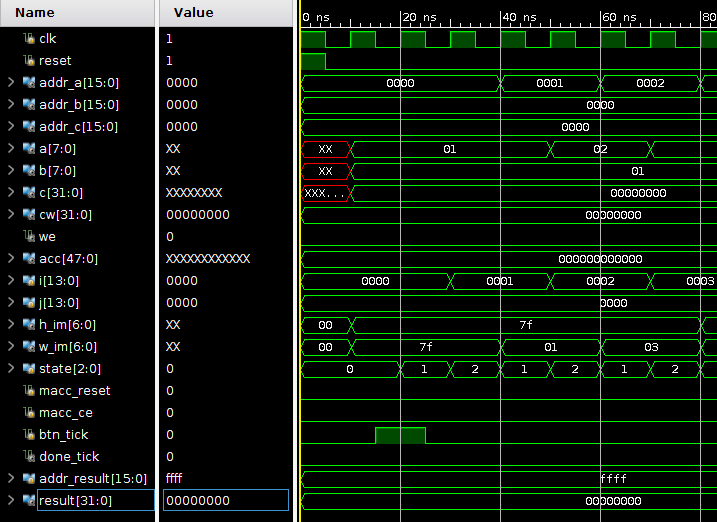
\includegraphics[scale=0.5]{behavioral_simulation}
  \caption{Behavioral Simulation of Transposed Convolution Module}
  \label{fig:behavioral_simulation}
\end{figure}

\clearpage %force the next chapter to start on a new page. Keep that as the last line of your chapter!

% Project Specifications

\chapter{Optimization}

TODO

\clearpage %force the next chapter to start on a new page. Keep that as the last line of your chapter!

% uncomment what you need.
%\input{chapters/projectSpec.tex}
%\input{chapters/methods.tex}
%\input{chapters/theory.tex}
%\input{chapters/solution.tex}
% Conclusions

\chapter{Conclusions and Future Work}

This section concludes the project by briefly discussing possible optimization methods.
As mentioned before, the main goal of the design was simplicity, so many optimizations were not applied.
The main bottleneck in the current design, as in many computing systems, is the I/O bandwidth. During
each clock cycle, only one unit of data is read, which is rather inefficient. Therefore, most of the
optimizations are focused on improving I/O efficiency.

The first obvious optimization is to transfer all weight data from Dual-SPI Flash to the \gls{psram} once
the \gls{fpga} is configured. Weights will be loaded from the \gls{psram} subsequently, which has a parallel
interface and will result in much faster loading of weights.
Burst transfer can be used to read data from \gls{psram} and further reduces I/O latency. This is done by
placing the starting address on the address bus, a fixed amount of data is then read repeatedly in a single
``burst''.

Another optimization mentioned is to widen the data buses connected to the \gls{psram}. Current the
data address of input buffer is only 8-bit. This can be increased to 32-bit or even more. Multiple data
can be loaded at the same time and calculation can be performed in parallel on these data. The current
design is highly sequential and only utilizes around $15\%$ of the \gls{dsp} slices.

Yet another optimization is to further introduce several small caches using distributed RAM. These caches
are implemented using \glspl{lut} and are faster than \glspl{bram}, i.e., they can be read asynchronously.
Once inputs and weights are loaded into these caches, more parallelism can be achieved,
making use of more \gls{dsp} slices.

Finally, on an \gls{fpga} chip with more \gls{bram} capacity, layer-level parallelism can be exploited, i.e.,
several layers can be calculated at the same time. This invovles modifying the current ring structure and
forward data to subsequent layers in a single pass. Each layer will work on its input concurrently, but
some global coordination and scheduling is needed in order to avoid data overrun.

\clearpage %force the next chapter to start on a new page. Keep that as the last line of your chapter!


% Sample content to demonstrate LaTeX command. You will likely delete this line and the 
% next \input{sample/*} lines. You are also safe to delete the sample/ folder and its
% content once you refershed your LaTeX skills. Also check the appendix samples.
%\input{sample/1content.tex}
%\input{sample/2lorem.tex}
%\input{sample/3graph.tex}

%----------------------------------------------------------------------------------------
%	BIBLIOGRAPHY REFERENCES
%----------------------------------------------------------------------------------------

\input{style/biblio.tex}

%----------------------------------------------------------------------------------------
%	APPENDICES 
%----------------------------------------------------------------------------------------

\input{style/appendix.tex}
%force smaller vertical spacing in table of content
%!!! There can be some fun depending if the appendices have (sub)sections or not :D
% You will have to play with these numbers and eventually add the \vspace line  before 
% some \chapter and force another number.
% To add more fun, time to time the table of content get wrong after a build :(
\addtocontents{toc}{\vspace{11pt}}
\pretocmd{\chapter}{\addtocontents{toc}{\protect\vspace{-24pt}}}{}{}

\liite{1}% This is a hack to have right page numbering for each appendix. Make sure to 
	 % use a unique number for each appendix.
% Appendix 
% And demonstrate text references and bibliography references in appendix

\chapter{Appendix: Code Listing of Transposed Convolution Module}\label{appx:verilog_listing}

\begin{code}
  \inputminted{verilog}{code/transposed_convolution.v}
  \captionof{listing}{Implementation of Transposed Convolution}
  \label{code:transposed_convolution}
\end{code}

\clearpage %force the next chapter/appendix to start on a new page. Keep that as the last line of your appendix!

% % Appendix 
% And demonstrate text references and bibliography references in appendix

\chapter{Appendix: Code Listing of Transposed Convolution Module}\label{appx:verilog_listing}

\begin{code}
  \inputminted{verilog}{code/transposed_convolution.v}
  \captionof{listing}{Implementation of Transposed Convolution}
  \label{code:transposed_convolution}
\end{code}

\clearpage %force the next chapter/appendix to start on a new page. Keep that as the last line of your appendix!
% Sample content to demonstrate appendix in LaTeX. You
% are safe to delete this lines (and the next samples) once you refreshed your LaTeX 
% skills (and safe to delete the sample folder and all its file too).

% \addtocontents{toc}{\vspace{11pt}}%fix vertical space for Table of Content
% \liite{2}
% \input{sample/Xappendix2.tex}

% \addtocontents{toc}{\vspace{11pt}}
% \liite{3}
% \input{sample/X_R_example.tex}


%----------------------------------------------------------------------------------------
%	THIS IS THE END 
%----------------------------------------------------------------------------------------
\end{document}
